\chapter{Case Study} \label{example}

In this chapter, I present a case study of my work, the summary of the validation of the UML PSSM standard about state machine semantics~\cite{tdk}. This work, co-authored by myself, was presented at the Scientific Students' Association Conference at the Budapest University of Technology and Economics in 2022.

I briefly present the \textit{Precise Semantics of UML State Machines} (PSSM) standard and its test suite (\autoref{sec:pssm}) and give an overview of our approach for validating the conformance of the standard and the test suite, emphasizing the role of the simulation framework (\autoref{sec:overview}). I also detail the validation through an example test case (\autoref{sec:example}).

\section{Precise Semantics of UML State Machines}\label{sec:pssm}

The \emph{Unified Modeling Language} (UML)~\cite{uml} is a general-purpose modeling language -- developed by the \emph{Object Management Group} (OMG) -- that is widely used in the model-based systems engineering domain to describe the behavior and structure of systems. UML provides numerous types of diagrams for visualizing different aspects of systems. \emph{State Machine Diagrams} and \emph{Activity Diagrams} are behavioral diagrams, whose purpose is to describe \emph{how} a component behaves in certain situations.

Base UML does not specify precisely the operational semantics of the behavior models. The \emph{Precise Semantics of UML State Machines} (PSSM)~\cite{pssm} is a follow-up specification for a subset of UML elements, refining their execution semantics. PSSM does not only define the semantics textually, but it also provides a \textit{Test Suite} containing 103 test cases grouped into 18 different packages based on which part of the semantics they test. The tests were manually created by experts based on 113 requirements extracted from the UML specification.

Every \textit{test case} consists of a \textit{test model}, the received \textit{events}, and the expected \textit{execution traces}.

The Test Suite in the standard has two main goals:
\begin{itemize}
    \item It explicitly details the possible executions of the test models. These examples make the standard \textit{more understandable}, so engineers can earn a deeper understanding of the modeling language semantics.
    \item The test models and the expected execution traces can be used for the \textit{conformance-checking} of modeling tools. If a modeling tool yields exactly the same sets of execution traces for the test models, the tool \textit{may} conform with the PSSM semantics. Of course, this approach does not \textit{prove} full tool conformance, but with the appropriate selection of test models, in practice, it can provide a strong enough guarantee.
\end{itemize}

\section{Overview}\label{sec:overview}

The validation workflow consists of the following steps. First, the high-level PSSM models are transformed into Gamma models preserving the semantics. The benefit of the Gamma modeling language is that it has precise formal semantics, and Gamma already provides a model transformation into XSTS models. Then, the Gamma models are transformed into XSTS models, the XSTS model is split, and the execution traces are generated with the simulator, in \textit{exhaustive} mode.

The overview of the PSSM validation workflow is shown in \autoref{fig:pssm-val-overview}. The exact steps in the figure are the following.

$\cir{1}$ The textual \textit{PSSM Semantics} defines implicit components (e.g., dispatcher) which are modeled as Gamma statecharts. These components (\textit{Common Gamma Components}) are general PSSM components, i.e., they are reusable for every specific test model.

$\cir{2}$ The concrete \textit{PSSM Test Model} is modeled as Gamma components (statecharts, doActivities) resulting in the \textit{Gamma Test Model}. (Note, that step $\cir{2}$ is manual but \textit{systemmatic}, so it could be automated as a model transformation.)

$\cir{3}$ Then, the \textit{Common Gamma Components} and the \textit{Gamma Test Model} are composed into one system resulting in the \textit{Gamma Composite Test Model}.

$\cir{4}$ The \textit{Gamma Composite Test Model} is transformed into an \textit{XSTS Model} using the existing Gamma-to-XSTS model transformation.

$\cir{5}$ Then, splitting is applied on the \textit{XSTS Model}, resulting in the \textit{Split XSTS Model}.

$\cir{6}$ Finally, the simulator traverses every execution trace of the \textit{Split XSTS Model} using the \textit{exhaustive} simulation mode, resulting in the final \textit{Execution Traces}.

\begin{figure}[ht]
	\centering
	\includesvg[inkscapelatex=false, height=0.9\textheight, keepaspectratio]{figures/pssm-val-overview.svg}
	\caption{Overview of the PSSM validation workflow.}
	\label{fig:pssm-val-overview}
\end{figure}

\section{Example}\label{sec:example}

In this section, I demonstrate the capabilities of the PSSM validation workflow through an example test case, Behavior 003-B~\cite{pssm}. I detail the test model, the expected execution trace defined in the test case, and the actual execution traces found by the \textit{exhaustive} simulator. I also compare them and draw conclusions about the difference and the usability of the simulator.

\subsection{Test Model}

The Target State Machine of the test is shown in \autoref{fig:pssm-003b-sm}. After instantiation, the initial RTC step takes the State Machine into the \emph{wait} state, in which it will stay until a \emph{Start} signal is received. Upon receiving the Start signal, it enters \emph{S1}, which has an entry behavior tracing \verb|S1(entry)|. After the entry behavior has finished, the state's doActivity is started asynchronously. \textit{S1} has a completion transition to \emph{FinalState1}, which will only fire upon successful completion of the doActivity. The test is only considered successful if it sends the \emph{testEnd} signal by firing transition \textit{T3}.

\begin{figure}
    \centering
    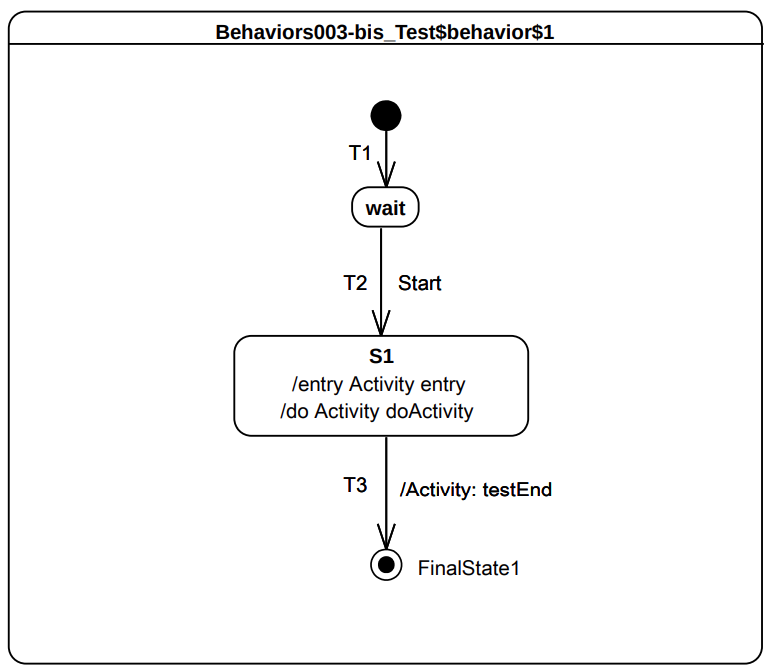
\includegraphics[width=0.6\textwidth]{figures/pssm-003b-sm.png}
    \caption{State Machine Diagram of Target component -- Behavior 003-B~\cite{pssm} test case.}
    \label{fig:pssm-003b-sm}
\end{figure}

The doActivity is shown in \autoref{fig:pssm-003b-do}. It begins its execution by taking a reference of \emph{this} (which is the State Machine's context) and duplicates the value using a \emph{fork} node. The separate branches go to two trace calls -- the first one traces \verb|S1(doActivityPartI)|, while the second one traces \verb|S1(doActivityPartII)|. Since there is an \emph{AcceptEventNode} between the two trace calls, the activity must receive a \emph{Continue} signal to execute the second trace call, finish execution and thus let the statechart reach its final state.

\begin{figure}
    \centering
    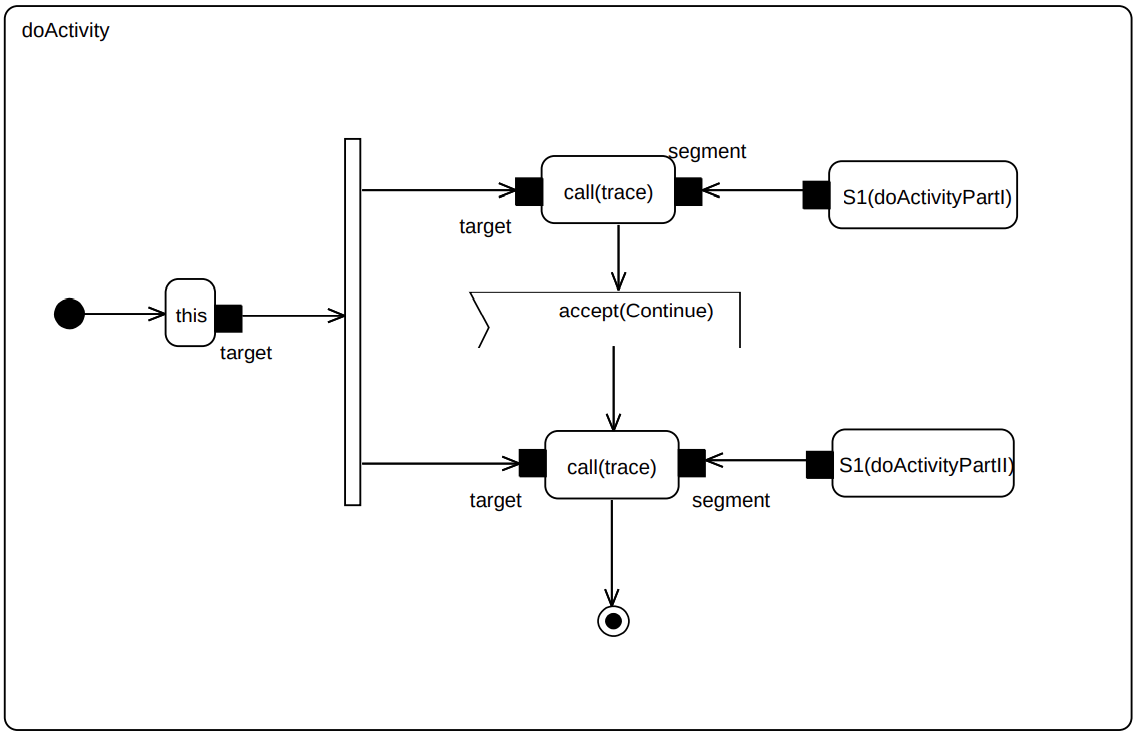
\includegraphics[width=0.8\textwidth]{figures/pssm-003b-do.png}
    \caption{Activity Diagram of S1's doActivity -- Behavior 003-B~\cite{pssm} test case.}
    \label{fig:pssm-003b-do}
\end{figure}

\subsection{Expected Trace}

The PSSM specification lists a single valid execution trace for this model:

\begin{itemize}
    \item \verb|S1(entry)|
    \item \verb|S1(doActivityPartI)|
    \item \verb|S1(doActivityPartII)|
\end{itemize}

The specification also provides the RTC steps during execution, which is shown in \autoref{tab:behavior_003b_rtc}. First, it fires transition \emph{T1} and enters state \emph{wait} as part of the \emph{initial RTC step}. Afterwards, a \emph{completion event} is generated for state \emph{wait}, as it does not have an entry behavior. Since there is no \emph{completion transition} from \emph{wait}, this event is discarded. Given, that the \emph{Start} signal is in the event pool, it triggers transition \emph{T2}. This transition takes the State Machine into state \emph{S1}, which asynchronously starts its doActivity Behavior. Afterward, the State Machine receives a \emph{Continue} signal, which is dispatched to the doActivity, enabling it to finish execution and let \emph{S1} generate a \emph{completion event}. Since S1 has a \emph{completion transition}, it fires, taking the State Machine into its final state, and sending a \emph{testEnd} signal, thus successfully completing the test.

\begin{table}[htbp]
\centering
\begin{tabular}{|l||l|l|l|}
\hline
\textbf{Step} & \textbf{Event pool} & \textbf{State Machine configuration} & \textbf{Fired transitions(s)} \\ \hline\hline
1    & {[}{]}              & {[}{]} - initial RTC step   & {[}T1{]}             \\ \hline
2    & {[}Start, \textbf{CE(wait)}{]} & {[}wait{]}                    & {[}{]}               \\ \hline
3    & {[}\textbf{Start}{]}         & {[}wait{]}                    & {[}T2{]}             \\ \hline
4    & {[}\textbf{Continue}{]}         & {[}S1{]}                    & {[}{]} -- doActivity RTC             \\ \hline
5    & {[}\textbf{CE(S1)}{]}         & {[}S1{]}                    & {[}T3{]}             \\ \hline
\end{tabular}
\caption{The run-to-completion steps for an execution of the Behavior 003-B~\cite{pssm} test case.}
\label{tab:behavior_003b_rtc}
\end{table}

\subsection{Deadlock of Test Model}\label{ssec:deadlock}

Upon closer examination of the PSSM semantics and the test case, we found that in certain situations the model can enter a deadlock\footnote{A state in which the State Machine does not have any more legal steps.} state before reaching its final state, which is not specified as a valid trace by the PSSM standard. The trace of that execution would look like the following:

\begin{itemize}
    \item \verb|S1(entry)|
    \item \verb|S1(doActivityPartI)|
    \item \textbf{(deadlock, final state not reached)}
\end{itemize}

The RTC steps for this trace are shown in \autoref{tab:behavior_003b_deadlock_rtc}. The beginning steps are the same up to the point of entering state \emph{S1}. Given the concurrent nature of doActivities, it is possible, that S1's doActivity does not reach its \emph{AcceptEventAction}, and thus does not register any \verb|EventAccepter| for the \emph{Continue} signal before the \emph{event dispatch} begins. In this case, since there are \textit{no} event accepters for the \textit{Continue} signal, it is \emph{discarded}. After this point, the doActivity will reach its trace action and \textit{AcceptEventNode}, thus registering a new event accepter for the \textit{Continue} signal. Since doActivities are only considered completed when they \emph{do not} have any event accepters registered and have no more actions to execute, the doActivity remains active, which prevents \textit{S1} from generating a completion event, thus the State Machine may never fire \textit{T3}. After this point, the State Machine has no more steps to take, thus the test case will never complete.

\begin{table}[htbp]
\centering
\begin{tabular}{|l||l|l|l|}
\hline
\textbf{Step} & \textbf{Event pool} & \textbf{State Machine configuration} & \textbf{Fired transitions(s)} \\ \hline\hline
1    & {[}{]}              & {[}{]} - Initial RTC step   & {[}T1{]}             \\ \hline
2    & {[}Start, \textbf{CE(wait)}{]} & {[}wait{]}                    & {[}{]}               \\ \hline
3    & {[}\textbf{Start}{]}         & {[}wait{]}                    & {[}T2{]}             \\ \hline
4    & {[}\textbf{Continue}{]}         & {[}S1{]}                    & {[}{]}             \\ \hline
\end{tabular}
\caption{The run-to-completion steps for a deadlocked execution of the Behavior 003-B~\cite{pssm} test case.}
\label{tab:behavior_003b_deadlock_rtc}
\end{table}

\subsection{Conclusion}

The possible deadlock of this model was found by the \textit{exhaustive} simulator which demonstrates the value of this approach and the usability of the simulator itself. The simulator traversed every possible execution of the model, aggregated the executions, and presented them graphically.

\autoref{fig:behavior003b-actual} shows the generated execution traces by tracking only the Target log variables: $V_{T_1} = \{ v_{\mathrm{log_{target}}}, v_{\mathrm{log_{doActivity}}} \}$. The simulator also found the execution trace of reaching the \emph{deadlock} state. This trace is refined in \autoref{fig:behavior003b-dispatcher}, which shows the generated execution traces by tracking the Target logs and the Dispatcher logs as well: $V_{T_2} = V_{T_1} \cup \{ v_{\mathrm{log_{dispatcher}}} \}$.

Note, that \autoref{fig:behavior003b-actual} and \autoref{fig:behavior003b-dispatcher} show the same execution traces, only with different granularity. In \autoref{fig:behavior003b-actual}, only the PSSM-level trace statements (modeled as Gamma log statements) are shown which also serves as an example for the back-annotation of the low-level simulation to the high-level. In \autoref{fig:behavior003b-dispatcher}, the execution traces contain more details demonstrating the customizable set of tracked variables.

\begin{figure}
\centering
\includesvg[inkscapelatex=false, height=200pt, keepaspectratio]{figures/behavior003b-actual.svg}
\caption{The actual execution traces of Behavior 003-B~\cite{pssm}, found by our approach with tracking variables $V_{T_1}$. The expected execution trace defined by PSSM is colored green, while the execution trace reaching a deadlocked state (discussed in \autoref{ssec:deadlock}) is colored red~\cite{tdk}.}
\label{fig:behavior003b-actual}
\end{figure}

\begin{figure}
\centering
\includesvg[inkscapelatex=false, width=\textwidth, keepaspectratio]{figures/behavior003b-dispatcher.svg}
\caption{The actual execution traces of Behavior 003-B~\cite{pssm}, found by our approach with tracking variables $V_{T_2}$. The nodes representing dispatcher interactions (discussed in \cite{tdk}) are filled with gray, in their label D denotes the dispatcher, SC denotes the statechart, and A denotes the activity. The deadlocked execution traces (discussed in \autoref{ssec:deadlock}) are colored red. The red nodes show the reasons for the deadlocks, i.e. that the statechart sends the ignore message to the dispatcher before the subscription of the activity~\cite{tdk}.}
\label{fig:behavior003b-dispatcher}
\end{figure}
